% You should title the file with a .tex extension (hw1.tex, for example)
\documentclass[11pt]{article}

\usepackage{hyperref}
\usepackage{amsmath}
\usepackage{mathtools}
\usepackage{amssymb}
\usepackage{wrapfig}
\usepackage{fancyhdr}
\usepackage{tikz-qtree}
\usepackage{tikz-qtree-compat}
\usepackage[normalem]{ulem}
\usepackage{tikz}
\usepackage{systeme}
\usepackage{graphicx}
\DeclareMathOperator*{\argmin}{argmin}
\DeclareMathOperator*{\argmax}{argmax}
\usepackage{bm}

\oddsidemargin0cm
\topmargin-2cm     %I recommend adding these three lines to increase the 
\textwidth16.5cm   %amount of usable space on the page (and save trees)
\textheight23.5cm  

\newcommand{\question}[2] {\vspace{.25in} \hrule\vspace{0.5em}
\noindent{\bf #1: #2} \vspace{0.5em}
\hrule \vspace{.10in}}
\renewcommand{\part}[1] {\vspace{.10in} {\bf (#1)}}

\newcommand{\myname}{Sean Bittner}
\newcommand{\myandrew}{srb2201@columbia.edu}
\newcommand{\myhwnum}{12}

\setlength{\parindent}{0pt}
\setlength{\parskip}{5pt plus 1pt}
 
\DeclarePairedDelimiter\abs{\lvert}{\rvert}%
 %
\pagestyle{fancyplain}
\rhead{\fancyplain{}{\myname\\ \myandrew}}

\begin{document}

\medskip                        % Skip a "medium" amount of space
                                % (latex determines what medium is)
                                % Also try: \bigskip, \littleskip

\thispagestyle{plain}
\begin{center}                  % Center the following lines
{\Large Draft of new V1 section} \\
Sean Bittner, Agostina Palmigiano \\
November 24, 2020 \\
\end{center}

\section{Exploratory analysis of V1 with EPI produces a novel theory}\label{results_V1}
Dynamical models of excitatory (E) and inhibitory (I) populations with supralinear input-output function have succeeded in explaining a host of experimentally documented phenomena.
In a regime characterized by inhibitory stabilization of strong recurrent excitation, these models give rise to paradoxical responses \cite{tsodyks1997paradoxical}, selective amplification  \cite{goldman2009memory, murphy2009balanced}, surround suppression \cite{ozeki2009inhibitory} and normalization \cite{rubin2015stabilized}. 
Despite their strong predictive power, E-I circuit models rely on the assumption that inhibition can be studied as an indivisible unit. 
However, experimental evidence shows that inhibition is composed of distinct elements -- parvalbumin (P), somatostatin (S), VIP (V) --
composing 80\% of GABAergic interneurons in V1 \cite{markram2004interneurons, rudy2011three, tremblay2016}, and that these inhibitory cell types follow specific connectivity patterns (Fig. \ref{fig:SV_flip}A) \cite{pfeffer2013inhibition}.
Recent theoretical advances \cite{litwin2016inhibitory, GarciaDelMolino2017, Chen2019},  have only started to address the consequences of this multiplicity in the dynamics of V1, strongly relying on linear theoretical tools. 
Here, we use EPI to elucidate the mechanisms of neuron-type stability in V1 at different levels of contrast.

We consider contrast responses of a nonlinear dynamical V1 circuit model (Fig. \ref{fig:Fig3}A) with a state comprised of each neuron-type population's rate $x = \left[x_E, x_P , x_S, x_V \right]^\top$.
Each population of neuron-type $\alpha$ receives recurrent input $\left(W f_r(x)\right)_\alpha$ from synaptic projections, where $W$ is the connectivity matrix and $f_r = \left[\cdot\right]_+^2$ is the rate nonlinearity.
Driven by a baseline input $\mathbf{b}$, the circuit evolves form an initial condition $\mathbf{x}(0)$ to a steady-state solution (Fig. \ref{fig:Fig3}B, solid).
When slow noise $\mathbf{\epsilon}$ is introduced, circuit activity fluctuates around this solution (Fig. \ref{fig:Fig3}B dashed), and the model is then a stochastic stabilized supralinear network (SSSN) \cite{hennequin2018dynamical} (see Section \ref{methods_V1}).
As contrast is enhanced, input to the E- and P-populations via $h^{(c)}$ increases causing the steady state solution (and fluctuations thereabout) to change  (Fig. \ref{fig:Fig3}C).
In this analysis, we consider $W$,$b$, and $h^{(c)}$ that have been fit to contrast responses in mouse V1 using the deterministic model (TODO cite, see Section \ref{methods_V1}).
As contrast changes, so does the degree of stochastic variability of each neuron-type (Fig. \ref{fig:Fig3}D).
Moreover, the circuit transitions into an inhibition-stabilized network (ISN) with increasing contrast (Fig. \ref{fig:Fig3}D inset).
While the ISN-regime and it's effects are well understood in E-I networks, it's role in the stability of this SSSN with inhibitory multiplicity has not been explored.

To study the role of inhibition stabilization in this network, we explore the changes in input 
\begin{equation}
\mathbf{z} = \begin{bmatrix} dh_E & dh_P & dh_S & dh_V \end{bmatrix}^{\top}
\end{equation}
resulting in each neuron-type's stability around it's mean rate.
The emergent property of ``neuron-type stability" for population $\alpha$  at contrast level $c$ is defined as 
\begin{equation}\label{eq:EP}
\begin{split}
\mathcal{X}(\alpha, c) ~~:~~  \mathbb{E}_{\mathbf{z}}\begin{bmatrix} dx_\alpha(\mathbf{x}; \mathbf{z},c) \end{bmatrix}  &~~=~~  0  ~~\triangleq~~ \bm{\mu}  \\ 
\text{Var}_{\mathbf{z}}\begin{bmatrix} dx_\alpha(\mathbf{x}; \mathbf{z},c) \end{bmatrix}  &~~=~~  \begin{bmatrix} 0.05^2 \end{bmatrix} ~~\triangleq~~ \bm{\sigma}^2 .
\end{split}
\end{equation}


\clearpage
\begin{figure}[h]
\caption{\small \textbf{A}.  Four-population model of primary visual cortex with excitatory (black), parvalbumin (blue), somatostatin (red), and VIP (green) neurons.   Some neuron-types largely do not form synaptic projections to others  (excitatory and inhibitory projections filled and unfilled, respectively).
\textbf{B}. EPI posterior $q_\theta(z \mid \mathcal{B}_{S-V})$ for S-V flipping. The obtained posterior is visualized as 500 samples from the inferred distribution colored by $\log(q_\theta(z))$. This posterior is bimodal and concentrated in planes $h^{(c)} > 0$ and $h^{(c)} < 0$ at distinct modes $z_1$ (black star) and $z_2$ (gray, star), respectively.  Bottom-left: Posterior predictive distribution of the emergent property statistics with respect to the constrained means (black, dashed line) and variances (gray, dashed lines at two standard deviations). 
\textbf{C}. Posterior predictive distribution of $d_{S,V}$ for each mode.  The $z_1$-mode produces V-to-S flipping with increasing contrast.
\textbf{D}. Model simulations at the mode $z_1$ at $c=0$ (solid) and $c=1$ (dashed). \textbf{E}. Mean system response at varying contrasts for $z_1$. Error bars show noise in rate. \textbf{F}. Plot of noise with contrast from E. Error bars are standard error measured across simulations.
 }\label{fig:Fig3}
\begin{center}
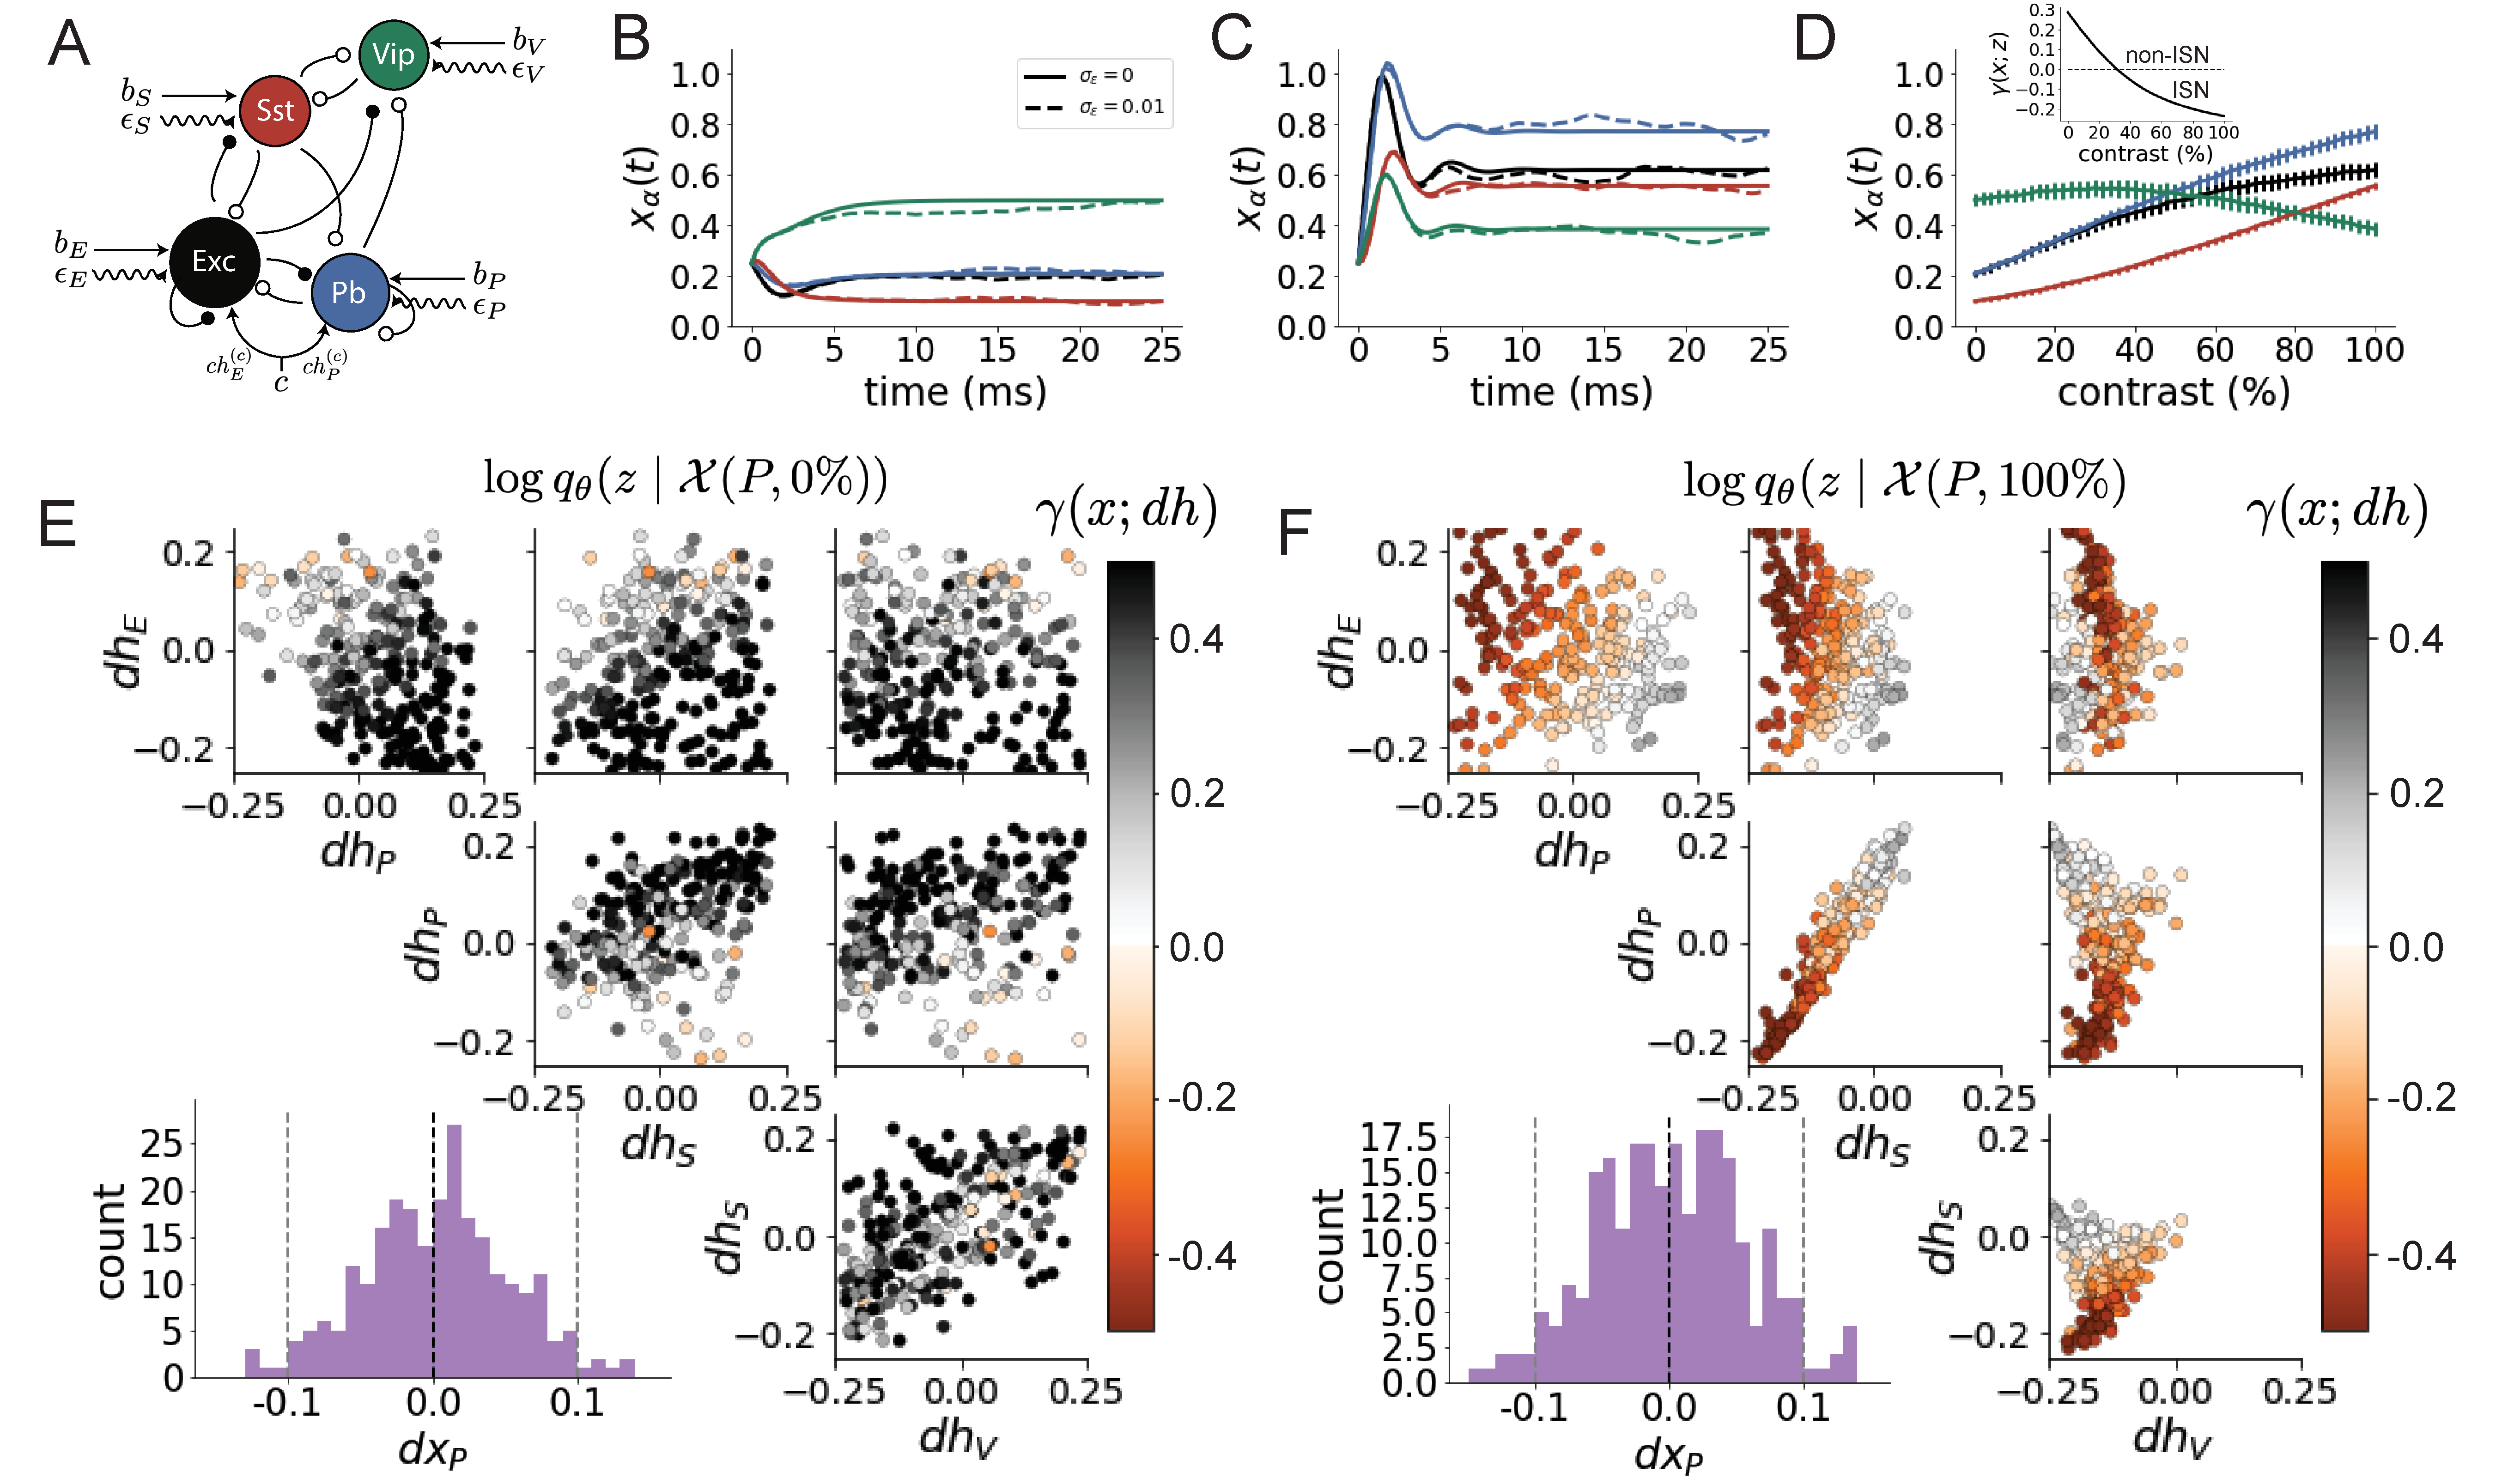
\includegraphics[scale=.18]{figs/Fig3/Fig3.pdf}
\end{center}
\end{figure}
\clearpage




\section{V1 Supplemental section}\label{methods_V1}

The dynamics are driven by the rectified and exponentiated sum of recurrent inputs $Wx$, external inputs $h$, and external noise:

\begin{equation}
\tau \frac{dx}{dt} = -x +Wf_r(x) + b + h + \epsilon
\end{equation}

where $\tau = 1 \text{ms}$, and $f_r(x) = \left[x \right]_+^2$.

The noise is modeled as an Ornstein-Uhlenbeck process:
\begin{equation}
\tau_{\text{noise}} d\epsilon_\alpha = -\epsilon_\alpha dt + \sqrt{2\tau_{\text{noise}}}\sigma_\alpha dB
\end{equation}

where $\tau_{\text{noise}}$ is slow at 5ms, $\sigma_\alpha =  0.01 $, and $dB$ is a standard Wiener process.

We considered the stability of this stochastic stabilized supralinear network using connectivity ($W$) and input ($b$ and $h^{(c)}$) parameters fit to the deterministic model (TODO cite)

\begin{equation}
W =  \begin{bmatrix} W_{EE} & W_{EP} & W_{ES} & W_{EV} \\
W_{PE} & W_{PP} & W_{PS} & W_{PV} \\
W_{SE} & W_{SP} & W_{SS} & W_{SV} \\
W_{VE} & W_{VP} & W_{VS} & W_{VV}  \end{bmatrix} = 
 \begin{bmatrix} .785 & -.102 & -1.24 & -.306 \\
.809 & -.100 & -.620 & -.264 \\
.833 & -.000128 & -.0000483 & -.742 \\
.708 & -.306 & -.452 & -.0000605 \\
 \end{bmatrix},
\end{equation} 

\begin{equation}
b =  \begin{bmatrix} b_E \\ b_P \\ b_S \\ b_V \end{bmatrix} =
 \begin{bmatrix} .590 \\ .504 \\ .515 \\ .670 \end{bmatrix} ,
\end{equation} 
and
\begin{equation} 
h^{(c)} = \begin{bmatrix} h^{(c)}_E \\ h^{(c)}_P \\ 0 \\ 0 \end{bmatrix} = 
\begin{bmatrix} .595 \\ .396 \\ 0 \\ 0 \end{bmatrix}.
\end{equation} 

This ISN coefficient $\gamma(x; z)$ is calculated by simulating 


The expectation and variance in the emergent property definition are taken over both the posterior distribution and the stochasticity of the SSSN:
\begin{equation}
= \mathbb{E}_{\mathbf{z}}\begin{bmatrix} dx_\alpha(\mathbf{x}; \mathbf{z},c) \end{bmatrix}  = \mathbb{E}_{\mathbf{z}\sim q_\theta} \left[ \mathbb{E}_{\mathbf{x} \sim p(\mathbf{x} \mid \mathbf{z})} \begin{bmatrix} x_\alpha(\mathbf{x}; \mathbf{z},c) - x_\alpha(\mathbf{x}; \mathbf{0},c) \end{bmatrix}\right].
\end{equation}

\begin{figure}[h]
\caption{\small SX 1
 }\label{fig:SX1}
\begin{center}
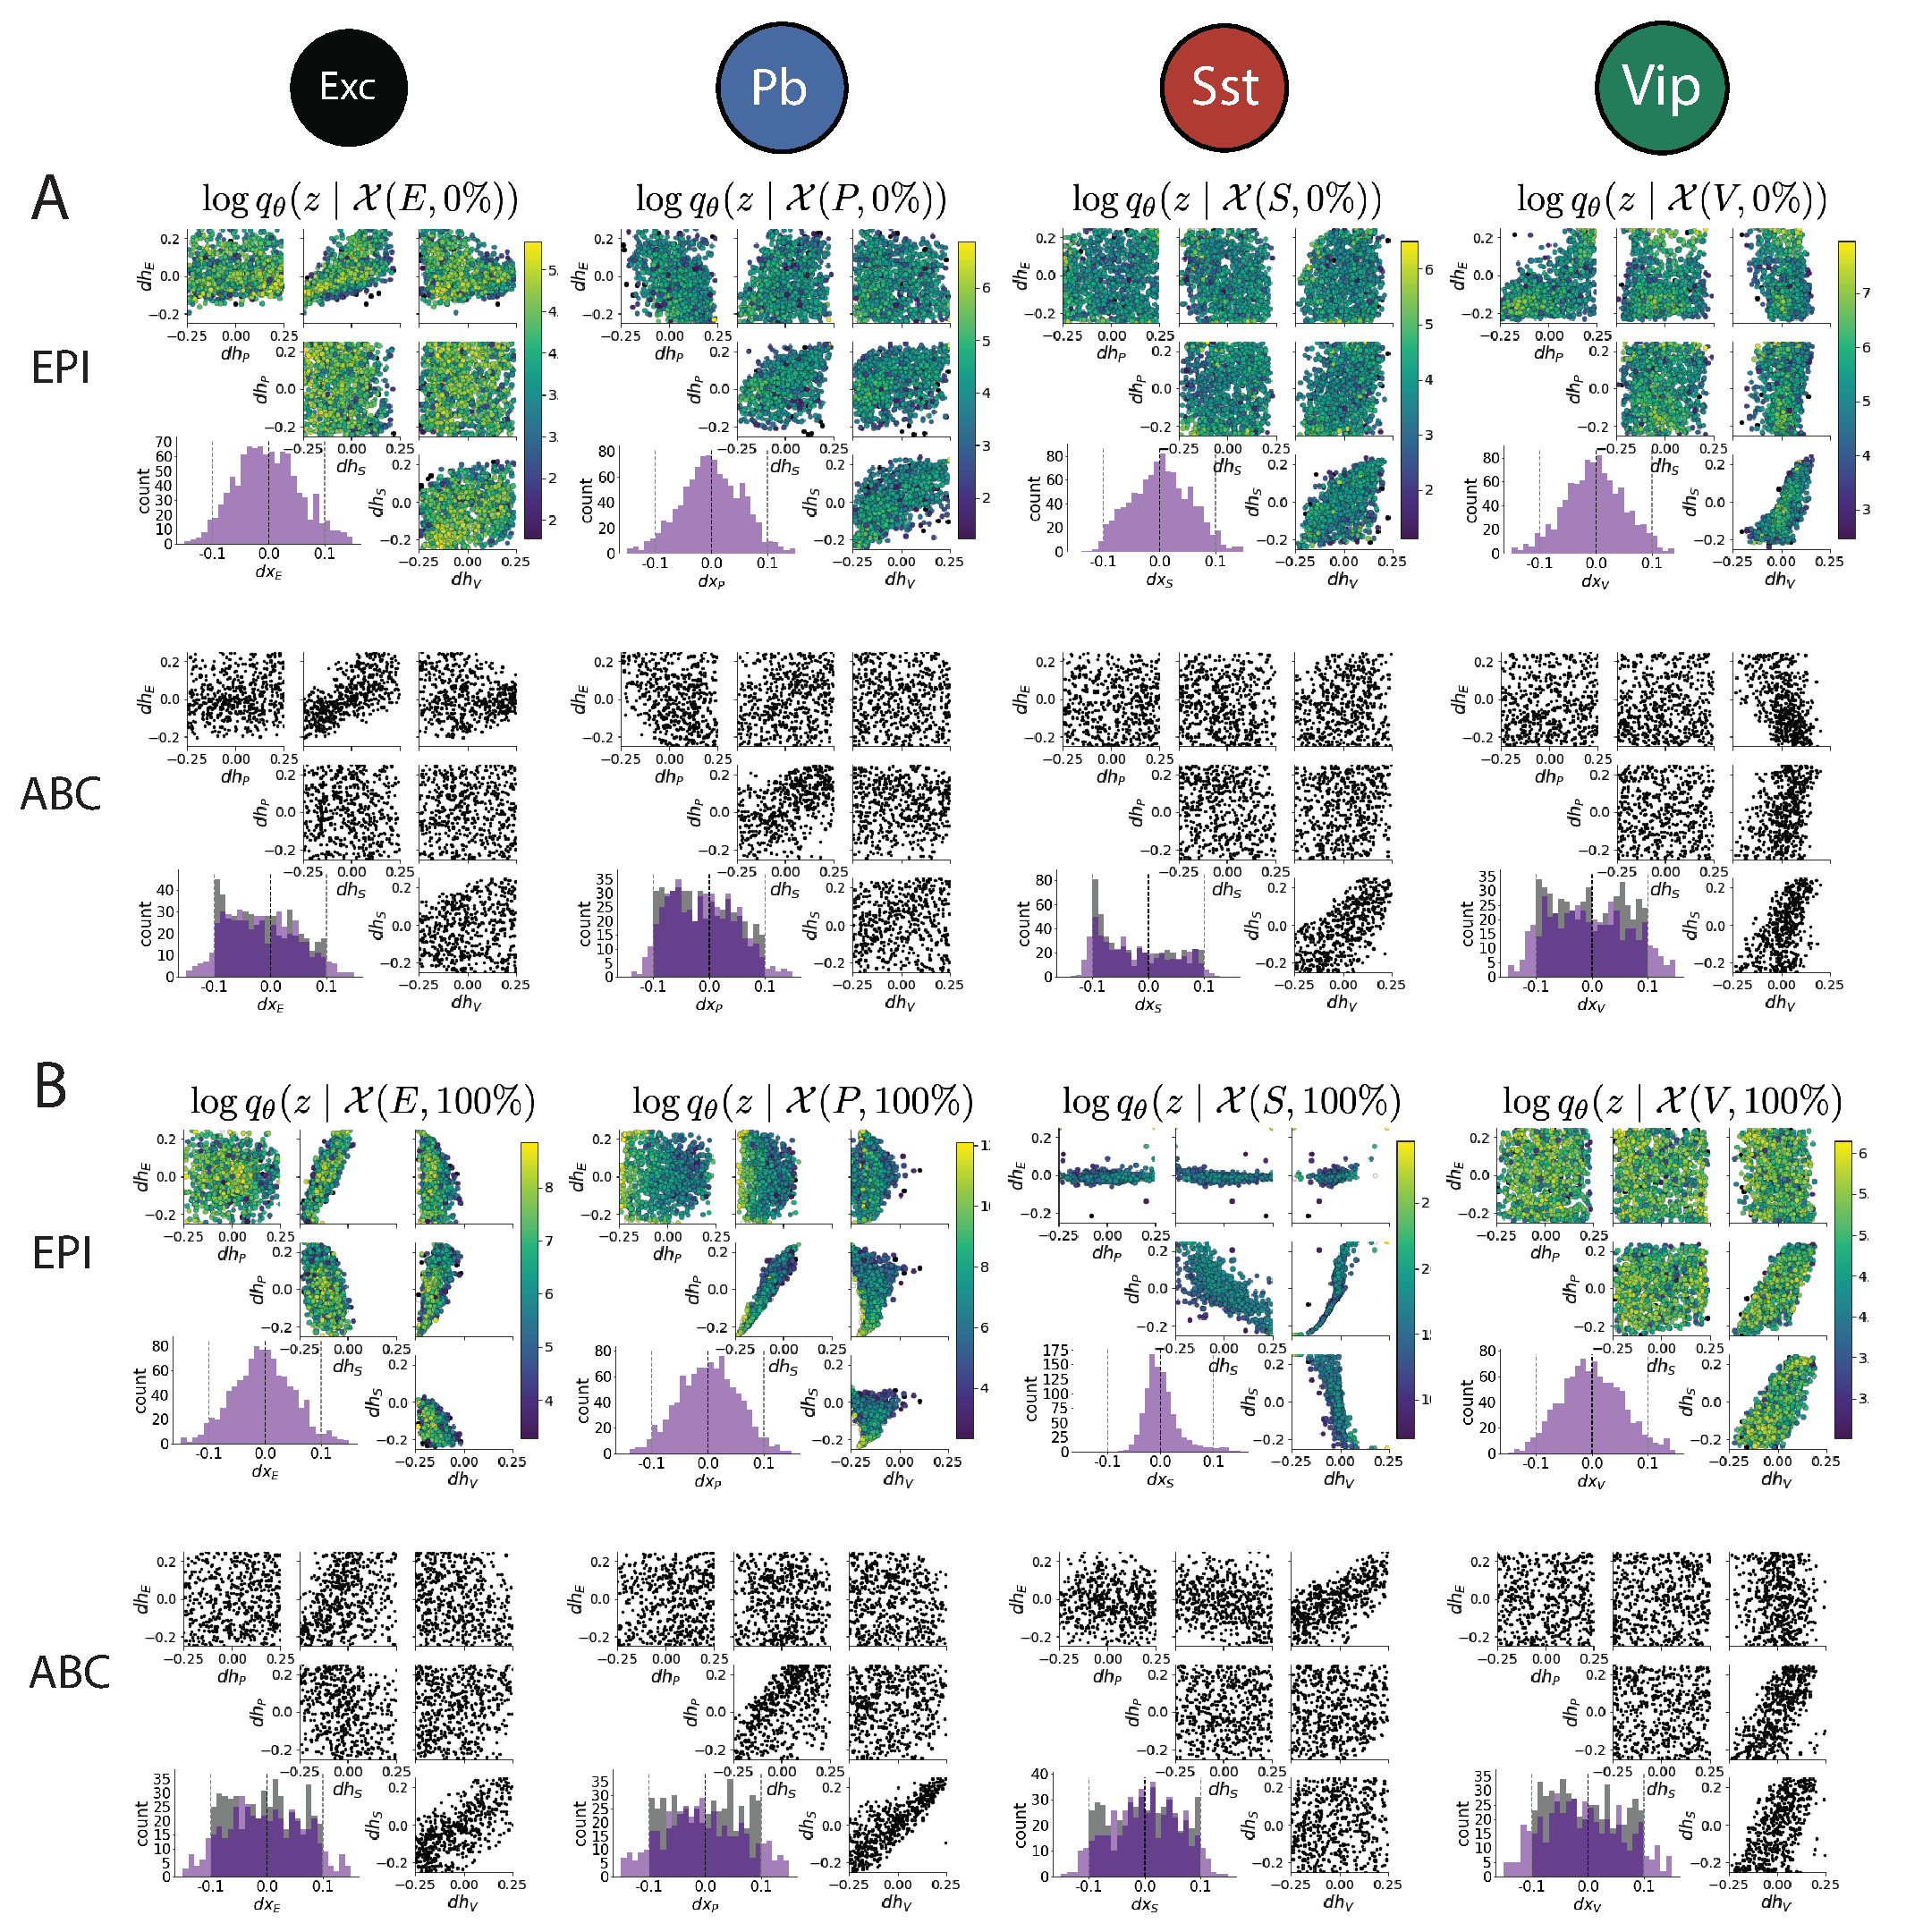
\includegraphics[scale=.5]{figs/FigSX/Fig_SX1.pdf}
\end{center}
\end{figure}

\begin{figure}[h]
\caption{\small SX 2
 }\label{fig:SX2}
\begin{center}
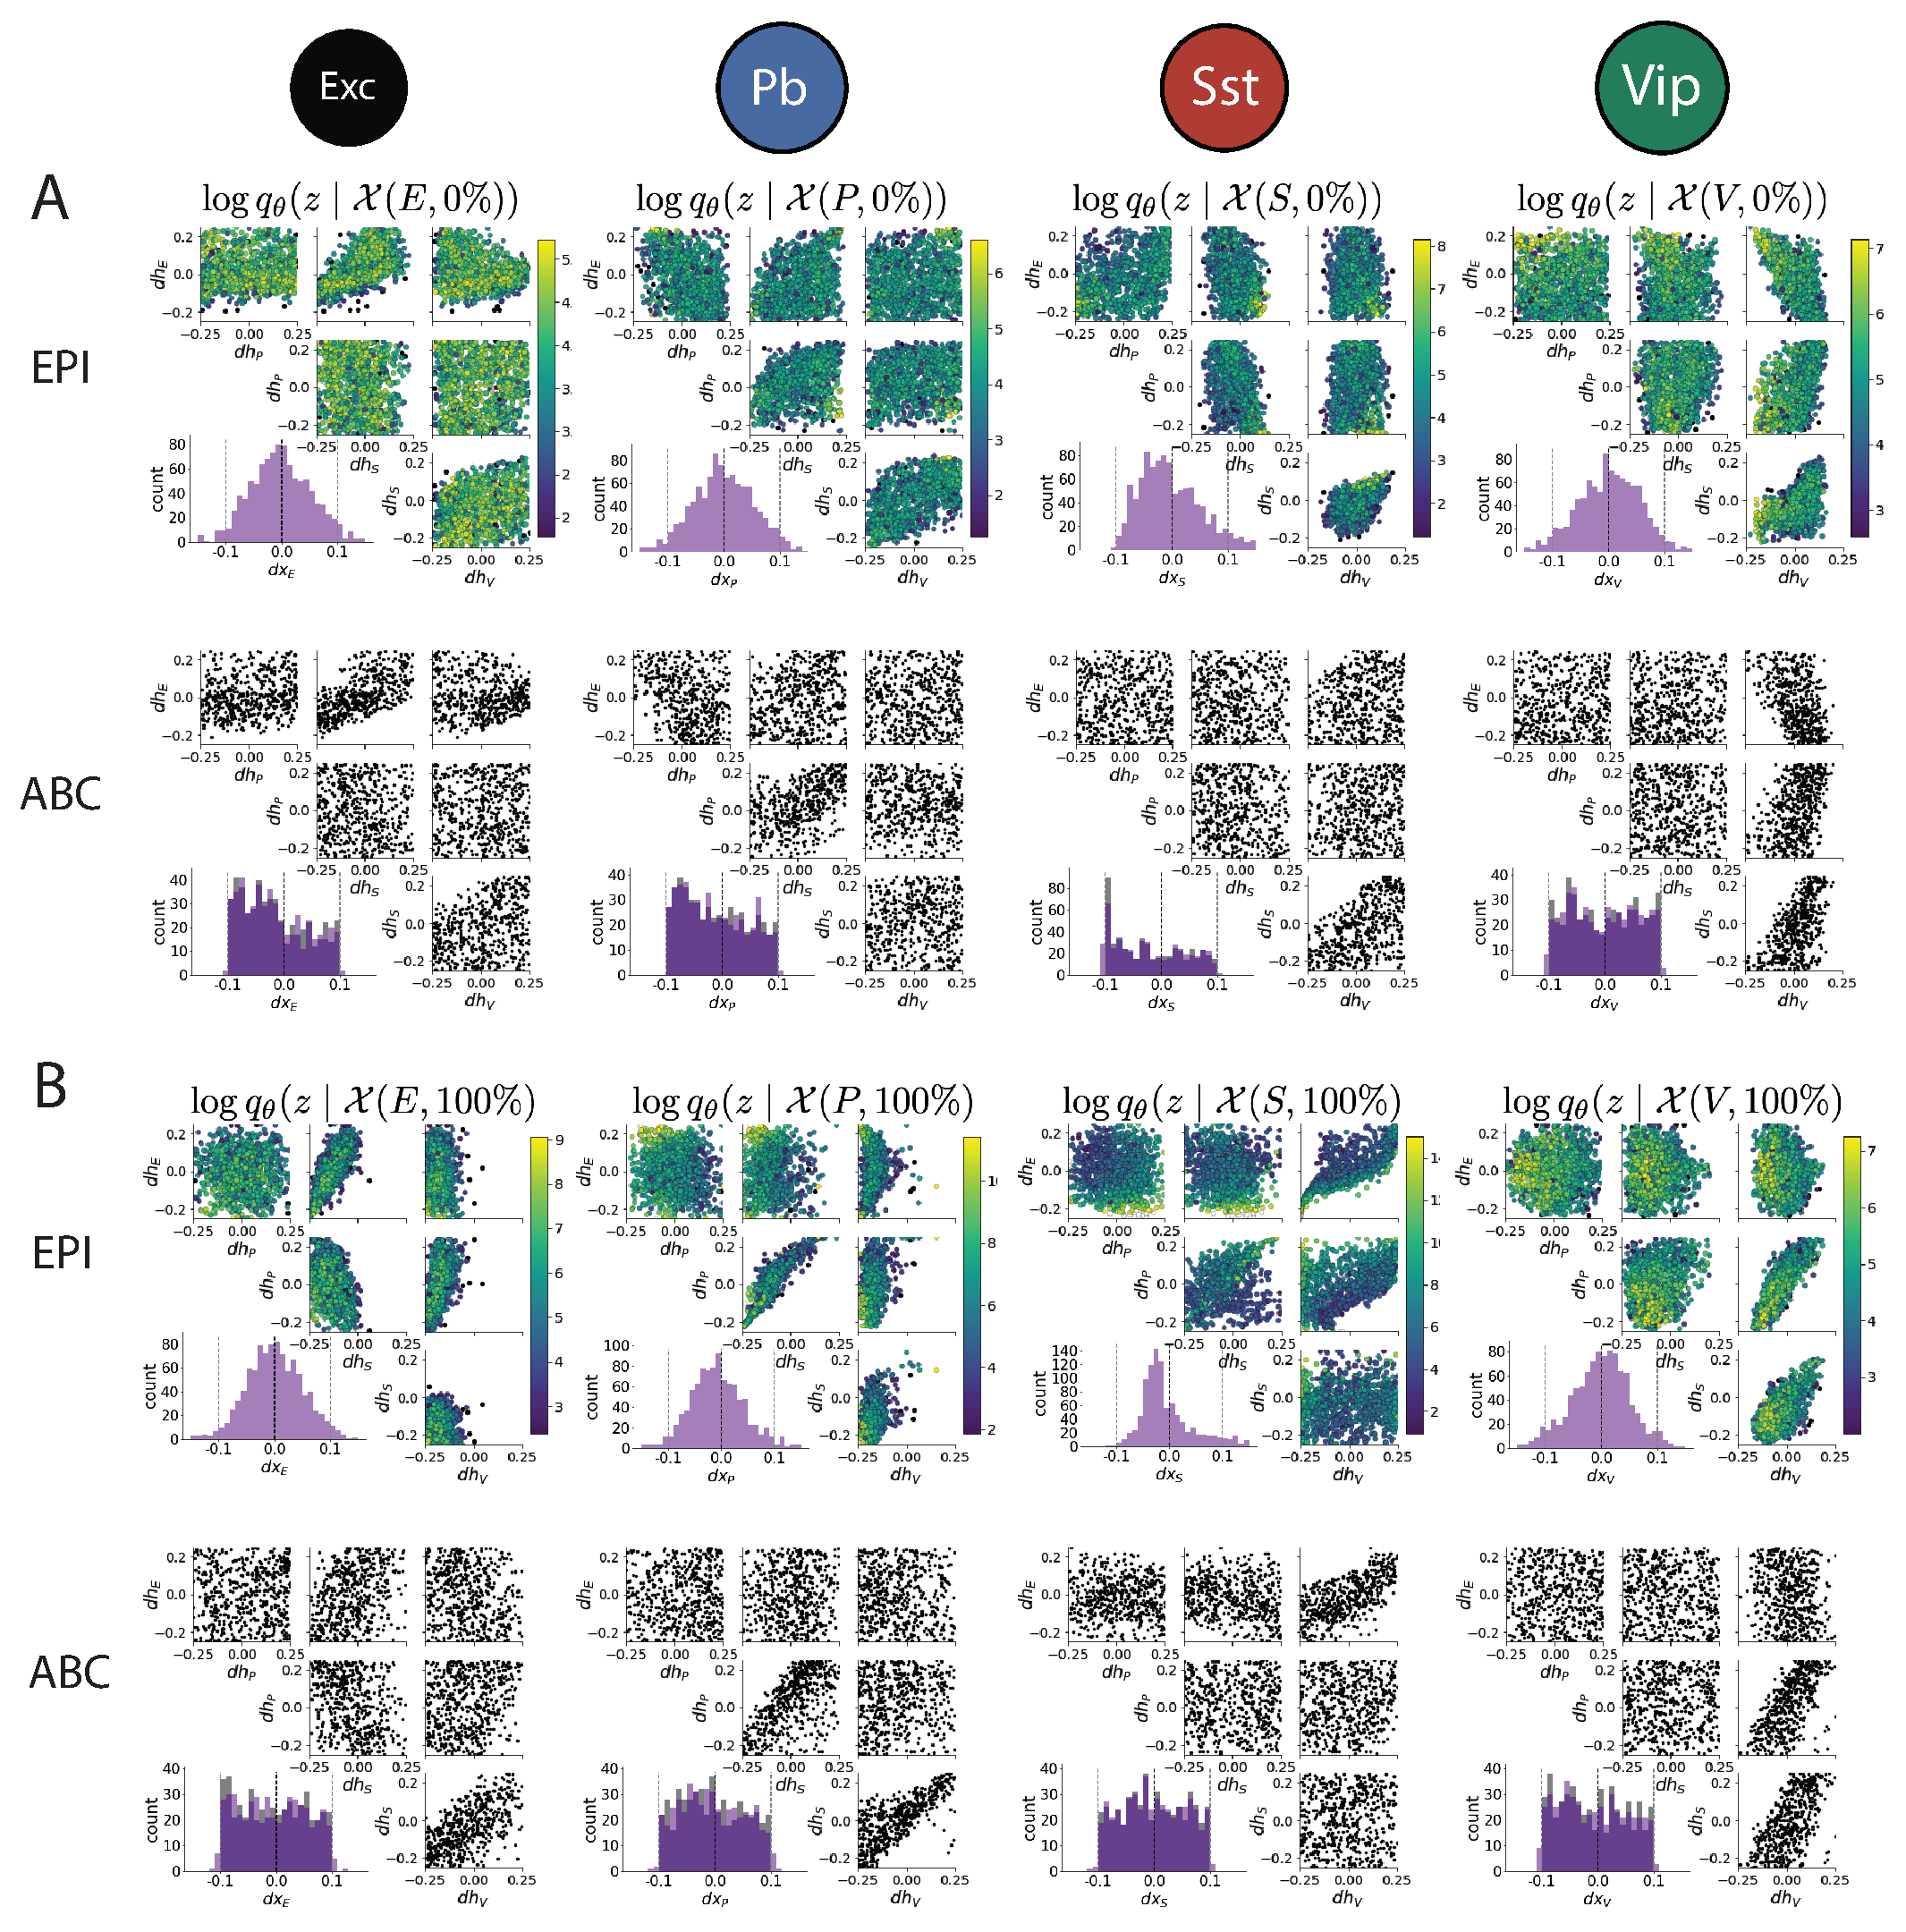
\includegraphics[scale=.5]{figs/FigSX/Fig_SX2.pdf}
\end{center}
\end{figure}


\bibliography{epi}
\bibliographystyle{unsrt}

 With this model, we are interested in the differential responses of each neuron-type population to changes in input $dh$. 
 Initially, we studied the linearized response of the system to input $\frac{dx_{ss}}{dh}$ at the steady state response $x_{ss}$, i.e. a fixed point. 
 All analyses of this model consider the steady state response, so we drop the notation $ss$ from here on.
 While this linearization accurately predicts differential responses $dx = \left[ dx_{E} , dx_{P} , dx_{S} ,dx_{V} \right]^\top$  for small differential inputs to each population $dh = \left[ 0.1 , 0.1 , 0.1 , 0.1 \right]^\top$ (Fig \ref{fig:V1_EPI}B left), the linearization is a poor predictor in this nonlinear model more generally (Fig. \ref{fig:V1_EPI}B right).  
 Currently available approaches to deriving the steady state response of the system are limited.

%\section{Stability analysis}
The input $h = b + dh$ is comprised of a baseline input  $b = \left[ b_E, b_P , b_S , b_V \right]^\top = \left[ 1, 1, 1 ,1.25 \right]^\top$  and a differential input $dh = \left[ dh_E , dh_P , dh_S , dh_V\right]^\top$ to each neuron-type population.  

We want to know the differential inputs $dh$ that maintain the steady state $x_{\alpha}$ for $\alpha \in \{E, P, S, V\}$. 
We see from Figure 1B that input to a single population in the recurrent circuit elicits a variety of responses across populations: E same, P up, S down, and V up.
We define the differential steady state $dx_{\alpha}$ as the change in steady state $x_{\alpha}$ when receiving input $h=b + dh$ with respect to the baseline $h = b$.
Maintaining the steady state of a neuron-type population amounts to the emergent property 
\begin{equation}
\mathcal{B}(\alpha, \sigma) ~~\triangleq~~ 
\mathbb{E} \begin{bmatrix} dx_{\alpha} \\ dx_{\alpha}^2 \end{bmatrix} ~~=~~ \begin{bmatrix} 0 \\ \sigma^2 \end{bmatrix}.\\
\end{equation}
In the following analyses, we chose $\sigma=0.25$.

\section{EPI agrees with ABC}
To get an idea of what distribution of parameters ($dh$) we should expect from EPI, we can use ABC to obtain a set of parameters related to the emergent property.  
We compare EPI to ABC with a rejection heuristic defined by the standard deviation of the differential responses $\sigma_{ABC}$
 \[f_{ABC}(dx_\alpha; \sigma_{ABC}) = |dx_\alpha| > 2\sigma_{ABC}.\]
 In other words, we ran ABC accepting parameters that generate differential responses within two standard deviations $\sigma_{ABC}=0.25$ of $dx_\alpha = 0$.
 In Figure 2, we see that the distributions obtained via EPI (colored by $\log q_\theta(z)$) are visually similar to those obtained via ABC (colored by $dx_\alpha$). \\
 
 \textbf{Figure 2}: EPI (left) vs ABC (right).  Arrows in EPI distribution indicate dimensions of maximal sensitivity at selected parameters $dh$. The importance of $v_S$ and $v_P$ are explained in section 4.2. \\

There are some subtle differences between the EPI and ABC distributions, but some difference is to be expected.
Rather than simply attributing these differences to imperfection of the EPI optimization routine, we consider the the effect of bias in $dx_\alpha$ from ABC (and lack thereof from EPI).

When $\epsilon > 0$ in ABC, the samples are \textit{not} from the posterior distribution.
For $\epsilon > 0$, the ``posterior" predictive means of ABC $\mathbb{E}_{ABC(\alpha, \sigma_{ABC})}\left[dx_\alpha \right]$ may be far from zero.
In Figure 3, we see that with ABC, there is an increasingly negative bias in $\mathbb{E}_{ABC(\alpha, \sigma_{ABC})}\left[dx_\alpha \right]$ for greater error tolerances across all neuron-types.  
Additionally with ABC, there is no precise control of the variance $\mathbb{E}_{ABC(\alpha, \sigma_{ABC})}\left[dx_\alpha^2 \right]$, which may be undesireable.

In contrast, the first and second moments of $dx_\alpha$ are controlled to a specified degree of accuracy (Figure 4).
The variances of each distribution of $dx_\alpha$ are close to their target value $0.25^2 = 0.0625$ (see variances next to histograms of Figure 4). 

\end{document}